\documentclass{report}
\usepackage[utf8]{inputenc}
\usepackage{graphicx}
\usepackage{natbib}
\usepackage[nottoc]{tocbibind}
\usepackage{multicol}
\usepackage[top=1.10in, bottom=1.10in, left=1.25in, right=1.25in]{geometry}
\usepackage{textcomp}
\usepackage{listings}
\usepackage{color} 
\usepackage{hyperref}
\usepackage{fancyhdr}
\usepackage[titletoc]{appendix}
\usepackage{quotchap}
\usepackage{placeins}
\usepackage{euscript}
\usepackage{fixmath}
\usepackage{amsmath}
\usepackage{systeme}

\begin{document}

    % Front page
    \thispagestyle{empty}

\begin{figure}[h!]
    \centering
    
\includegraphics[scale=0.35]{images/unimi.jpg}
    \label{fig:logo}
\end{figure}

\begin{center}
\large{UNIVERSITY OF MILAN}\vspace{2mm}\\
    \large{DEPARTMENT OF SCIENCE AND TECHNOLOGY}\vspace{2mm}\\
    \small{MASTER'S DEGREE IN COMPUTER SCIENCE}
\end{center}

\vspace{35mm}

\begin{center}
    \large{INTELLIGENT SYSTEMS}\vspace{2mm}\\
    \Large{\textbf{Survey Project on Convolutional Neural Networks}}\\
\end{center}

\vspace{40mm}

\begin{multicols}{2}
    \begin{flushleft}
        \large{Submitted to:}\vspace{1mm}\\
        \large{\textbf{Prof. Vincenzo Piuri}}\\
        \columnbreak
    \end{flushleft}
    \begin{flushright}
        \large{Submitted by:}\vspace{1mm}\\
        \large{\textbf{Vittorio Triassi}}\\
        \large{\textbf{938344}}\\
    \end{flushright}
\end{multicols}

\vspace{40mm}

\begin{center}
    ACADEMIC YEAR 2018-2019
\end{center}

\newpage
    
    % Index
    \renewcommand{\contentsname}{Index}
    \large{\tableofcontents}
    
    % Introduction
    \chapter{Introduction}

The aim of the following report is to debate about the technology of \textit{Convolutional Neural Networks} by collecting a number of papers published from 2015 until 2019 on most famous digital libraries. More specifically, ten papers will be presented and organized into chapters which contain different approaches to improve performances on the subject under examination. Each paper will be discussed and divided into two sections. The first one will deal with the proposed method, while the second one will cover experimental results and achievements. Finally, in the last chapter of our discussion, we will draw conclusions. Before going any further, an overview on CNNs should be provided.

\section{CNNs' Overview}

Convolutional Neural Networks are a type of Neural Networks that are widely used in computer vision. They have become very popular because they can extract several features from images and have a very good accuracy when it comes to deal with image classification and object recognition. Basically it is possible to extract complex features by learning them from low-level to high-level features. More specifically, we go from learning edges, dots and textures to shapes that have a semantic meaning.\\ \\
At  this  point,  we  might  ask  ourselves,  what  is  the  difference  between a  CNN  and a common Neural Network. First of all, a CNN assumes that its input is an image. Of course we might also provide something different than images, but generally, if we are interested in learning something that needs to take account of locality, there is a good chance that we will use a CNN. Otherwise it would be more useful to pick another type of network. A Convolutional Neural Network is made of something that we might define as building blocks. They all are layers but if we want to be more specific they are going to be \textit{Convolutional Layer, Pooling Layer} and \textit{Fully-Connected Layer}. The main difference between a CNN and an ordinary NN is that each neuron in a CNN is not connected to all the neurons in the previous layer. So, we do not have a fully-connected approach but shared weights that will allow our model to have much less parameters. The key element in CNNs is the filter, which sometimes is also called kernel or patch. It represents a small matrix that usually is of size $3 \times 3$ or $5 \times 5$. Its purpose is to perform the convolution operation, which is the core of this kind of network. This operation is a dot product between the filter and the input image and is performed in the convolutional layer. We slide this window from the left side of our image to the right side until we cover all the image bearing in mind what is the size of our original image for a possible padding. We end up with another matrix that represents the result of the convolution. In CNNs we generally want to learn many different filters and each of these is going to be more sensitive to a particular feature. It is important to point out that in CNNs we have also a third dimension that is the \textit{depth}. Thus, we have layers of size $width \times height \times depth$. Having said this, we come up with stacking these convolutional layers, and for a fixed number of these, we might decide whether or not stack a pooling layer, whose aim is to downsample the original image by controlling the overfitting and reducing the number of parameters. Even though it needs to be said that a lot of research support the idea that pooling is not that useful so in the end it is up to us. Finally we have the fully-connected layers that follow the same logic as an ordinary neural networks. That is, all the neurons are connected to the previous layer. A fully-connected layer is also called ``output layer'' and if we are dealing with a classification problem, it returns the class probabilities.


    
    % Papers
    \chapter{Cascaded Subpatch Networks for Effective CNNs}

{\small \textbf{Authors}\\
Xiaoheng Jiang, Yanwei Pang, \textit{Senior Member, IEEE}, Manli Sun, and Xuelong Li, \textit{Fellow, IEEE}\\ \\
IEEE TRANSACTIONS ON NEURAL NETWORKS AND LEARNING SYSTEMS\\VOL. 29, NO. 7, JULY 2018}

\section{Proposed Method}

In this first paper we are going to talk about a new way to perform the convolution operation. It has been noted that the classical convolution might not be as efficient as we might think. As we know, the convolution is usually performed as an element-wise multiplication between an input patch of the image and a filter of a fixed size $H \times W$. Here, the novel approach is to represent the filter used for the convolution through subpatches that have a smaller size than the original filter. Basically, rather than convolving one filter with the input image, we will go through a gradual decrease of the filter size until it becomes of size $1 \times 1$. In order to do so, each subpatch will be made of two filters. The first one will represent the spatial size $h \times w$, while the second one will be the scalar result of size $1 \times 1$. It is noted that the size of a subpatch is always smaller than its previous. For instance, if the original patch is $H \times W$, the first subpatch must be such that $H > h$ and $W > w$ and so on. The idea is to convolve the subpatch filter with the input patch and then, by taking the output of this operation we feed it through another patch until we end up having just one neuron. Doing so, we represent these cascaded subpatches through a pyramid. It is worth to show the difference between a classical convolution and the one proposed here. In Figure \ref{fig:01_1}, the classical convolution returns a scalar value. On the other hand, in Figure \ref{fig:01_2}, we start with a patch of size $H \times W$ and we wind up with a single neuron. In this way, a \textit{csconv} filter is created and it basically represents just one filter. If many of these csconv filters are stacked layer by layer, a CSNet is created.

\begin{figure}[h!]
    \centering
    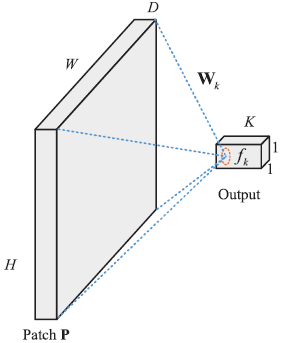
\includegraphics[scale=0.6]{images/01_1.png}
    \caption{Conventional convolutional filter}
    \label{fig:01_1}
\end{figure}

\FloatBarrier

\begin{figure}[h!]
    \centering
    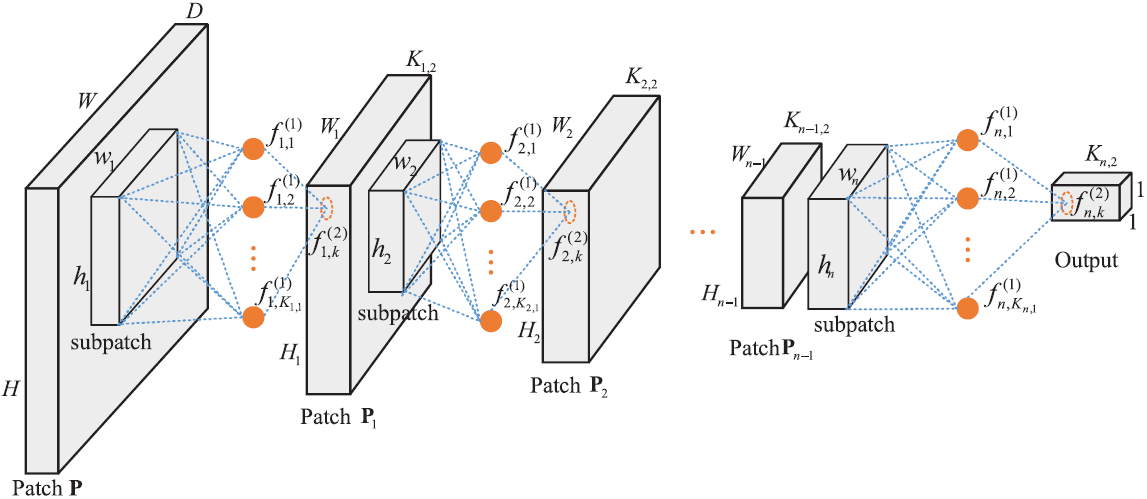
\includegraphics[scale=0.50]{images/01_2.png}
    \caption{n-stage \textit{csconv} filter $[(h_1 \times w_1, 1 \times 1), (h_2 \times w_2, 1 \times 1), ..., (h_n \times w_n, 1 \times 1)]$}
    \label{fig:01_2}
\end{figure}

\FloatBarrier

\section{Experimental Results}

In this section, experimental results are evaluated. First of all let us say that the proposed method has been evaluated on a few datasets. The datasets considered are: CIFAR10 \citep{CIFAR10and100}, CIFAR100 \citep{CIFAR10and100}, MNIST \citep{MNIST}, street view house numbers (SVHN) \citep{SVHN} and ImageNet 2012 \citep{ImageNet12}. Moreover, three different architectures of the CSNet have been used. The main difference among them is the number of the parameters, which is lower in the smallest architecture and it is progressively increased in the other two. Anyhow, it is worth mentioning the overall structure of these networks (Figure \ref{fig:01_3}). They are made of $n$ CSconv layers among which some max pooling layers have been added. The pooling operation has not been discussed in great detail yet, but it will be widely explained in another paper. Finally there is a softmax function whose aim is to return the class scores. As far as some of the tecniques employed in this work, we mention dropout, batch normalization and weight decay. Their purpose is basically to control overfitting and reduce the number of parameters. By testing this model on the mentioned datasets, very good results are obtained. This is translated into a real effectiveness of the cascaded subpatches method.\\

\begin{figure}[h!]
    \centering
    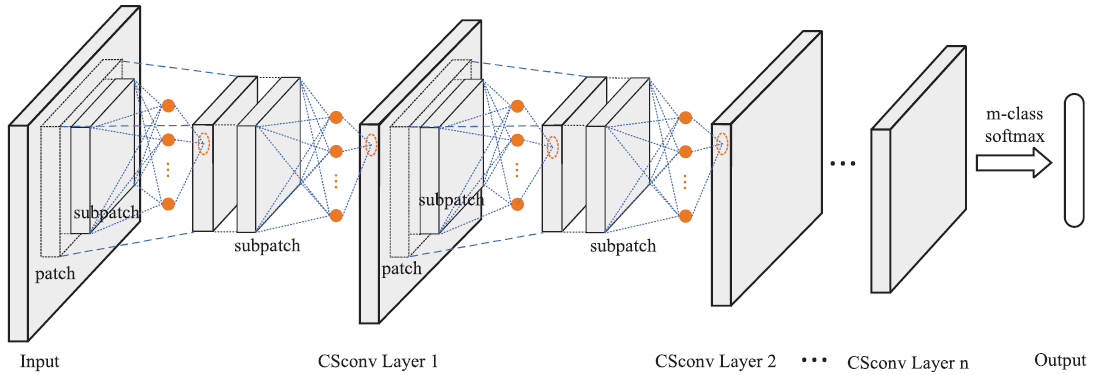
\includegraphics[scale=0.52]{images/01_3.png}
    \caption{Overall structure of CSNet}
    \label{fig:01_3}
\end{figure}

\FloatBarrier
    \chapter{Building Correlation Between Filters in Convolutional Neural Networks}

{\small \textbf{Authors}\\
Hanli Wang, \textit{Senior Member, IEEE}, Peiqiu Chen, and Sam Kwong, \textit{Fellow, IEEE}\\ \\
IEEE TRANSACTIONS ON CYBERNETICS\\VOL. 47, NO. 10, OCTOBER 2017}

\section{Proposed Method}

In this paper we will present a particular approach that aims at improving performance in CNNs through some observations on filters. It has already been explained how convolution generally works. Recall that we are looking for features to extract by learning some weights. The main idea here is to propose two different types of correlative filters. They are respectively \textit{static correlative filters} (SCFs) and \textit{parametric correlative filters} (PCFs). Before of going any further it would be worth understanding the basic idea for this study. Basically, it turns out from the paper that there is a link with neuroscience. More specifically, it has been observed that there are cells more sensitive to the light and others more sensitive to the darkness. Taking inspiration from that, we want to understand whether or not there is any connection between this idea and the way filters extract features from images in CNNs. Having said that, let us talk about the two proposed correlative filters approaches. As far as static correlative filters, four kinds of these filters are proposed and they are: opposite correlation, rotary correlation, scaling correlation and translational correlation. The idea is that we have some filters divided into \textit{master} and \textit{dependent} filters. If we let $m_{i,j}$ be the master and $d_{i,j}$ be the dependent filter, we end up with a few results. For instance, as concerns the \textit{opposite correlation} we will have that $d_{i,j} = -m_{i,j}$. In fact, if we take a look at letters (a) and (b) of Figure \ref{fig:02_1}, it is quite clear that in the dependent filter we obtain the exact opposite of the master filter. As far as the rotary correlation, for computational convenience, it has been considered only a rotation of 90°. On scaling correlation, a scaling equation is applied in order to reduce the size along both dimensions, width and height. Finally, as regards the translational correlation, which seems to be more complex, two filter have been used and they represent the part of the filter that goes upward and the other one that goes downward.\\

\begin{figure}[h!]
    \centering
    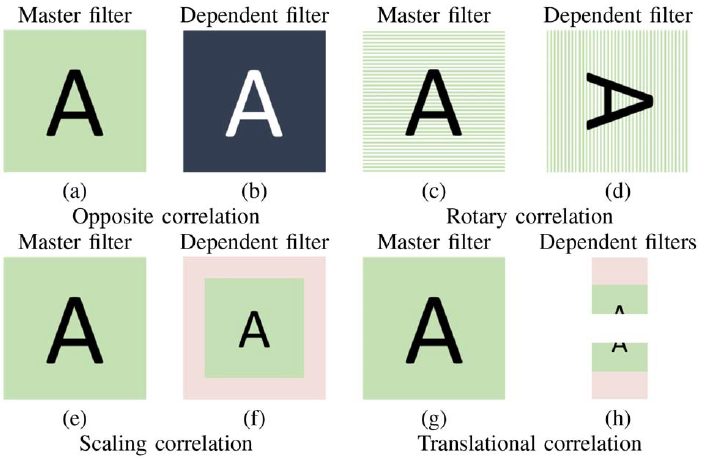
\includegraphics[scale=0.60]{images/02_1.png}
    \caption{Four kinds of proposed SCFs}
    \label{fig:02_1}
\end{figure}

\FloatBarrier

Another aspect that has been presented is how correlative filters are connected. It turns out that there are two strategies. They are the \textit{cross-map} connection and the \textit{within-map} connection. The first one is used with opposite and rotary correlations, while the second one is used on scaling and translational correlations. So far, it has been only said that there is a master and a dependent filter but it has not been shown how they work together. In Figures \ref{fig:02_2} and \ref{fig:02_3} is given an illustration of cross-map and within-map connections.

\begin{figure}[h!]
    \centering
    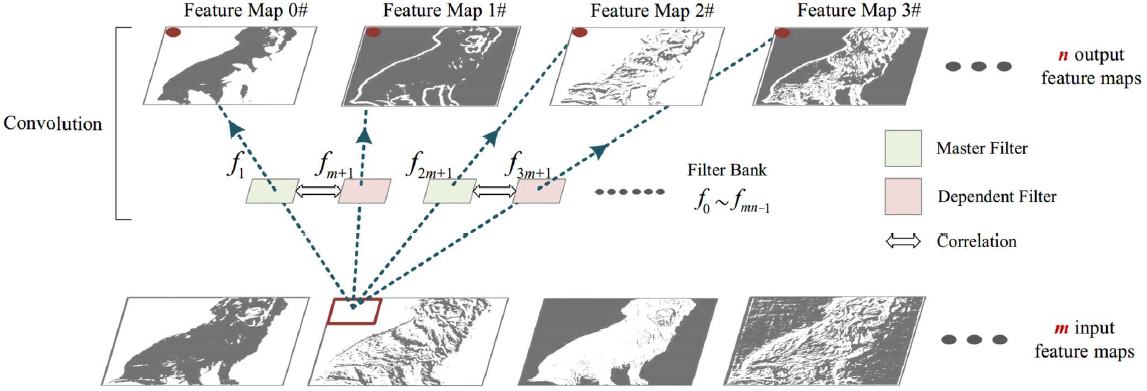
\includegraphics[scale=0.50]{images/02_2.png}
    \caption{Cross-map connection.}
    \label{fig:02_2}
\end{figure}

\FloatBarrier

\begin{figure}[h!]
    \centering
    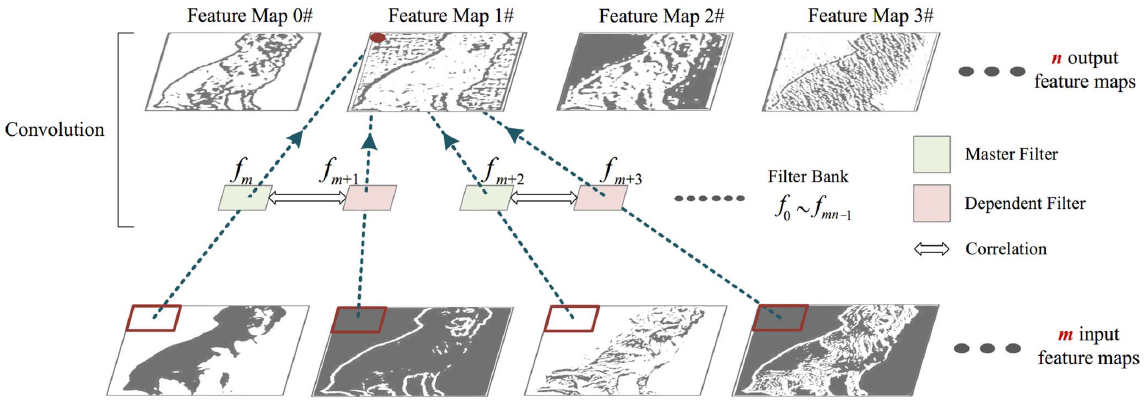
\includegraphics[scale=0.50]{images/02_3.png}
    \caption{Within-map connection.}
    \label{fig:02_3}
\end{figure}

\FloatBarrier

The main difference between the two is that in the cross-map connection we have a master that shares its feature map with a dependent filter but they refer to different output features. Instead, in the within-map connection, the master comes from a different input feature map but winds up in the same output feature map of other filters.\\ \\
Finally, there are parametric correlative filters (PCFs). They have been proposed in case we have not considered other correlations. The basic idea here is to use a correlation matrix which is gradually updated after the backward propagation. In fact it is possible to define this type of correlative filter like a fully-connected layer in an ordinary NN, so it follows the same logic. An illustration of how this correlative filter works is given in Figure \ref{fig:02_4}.\\

\begin{figure}[h!]
    \centering
    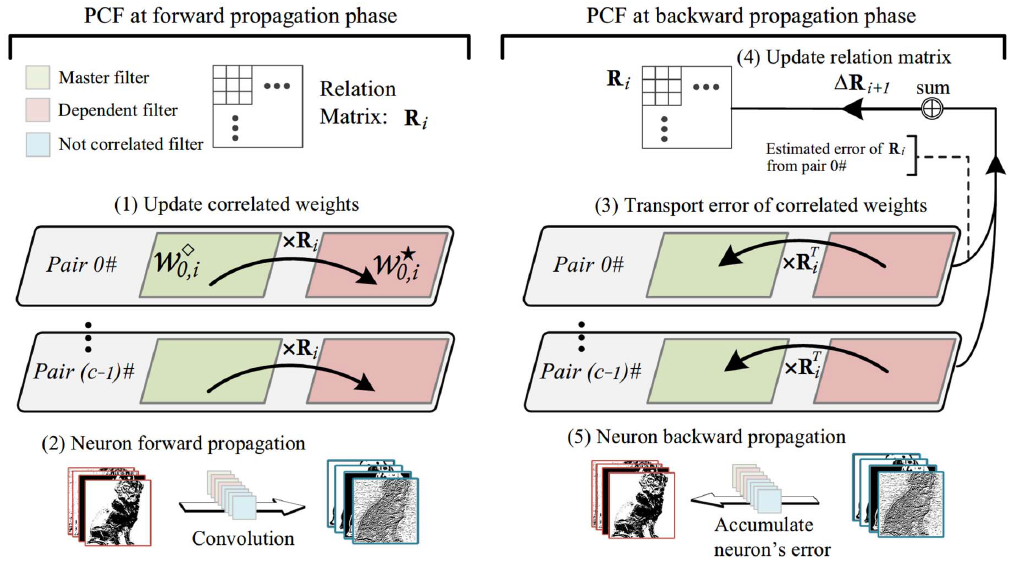
\includegraphics[scale=0.55]{images/02_4.png}
    \caption{PCFs training.}
    \label{fig:02_4}
\end{figure}

\FloatBarrier

\section{Experimental Results}

As far as the experimental results, five datasets have been used and they are: CIFAR10 \citep{CIFAR10and100}, CIFAR100 \citep{CIFAR10and100}, MNIST \citep{MNIST}, STL-10 \citep{STL10} and SVHN \citep{SVHN}. On some tests, data augmentation is performed. As it is the first paper in which we find this tecnique, it is worth saying a few words about it. Data augmentation is usually used when we do not have large datasets and we want to prevent overfitting as well. Basically, by performing simple operations such as cropping, flipping, etc. we can add more images for the same subject into our dataset. By doing so, if we run into some changes in light intensity for the given input image, we will still be able to classify correctly that image. Data augmentation is very useful and it allows to have better results on classification tasks and for this reason is widely used. Another tecnique applied in this paper is a classical regularization tecnique such as the dropout. In the end, by adopting the model SCF+PCF, it turns out that very good results are obtained on dataset previously mentioned with and without data augmentation. 

    \chapter{SparseConnect: regularising CNNs on fully connected layers}

{\small \textbf{Authors}\\
Qi Xu and Gang Pan\\ \\
ELECTRONICS LETTERS\\31st August 2017 Vol. 53 No. 18 pp. 1246–1248}

\section{Proposed Method}

In the following paper a novel approach to deal with the overfitting problem is proposed. First of all let us say something more about the overfitting that so far has not been explained in great detail. Overfitting is due to the inability of our model to behave well in the presence of data and more specifically it is generally caused by a high number of parameters.\\ \\
For this reason, the main goal in this paper is to propose an approach to deal with this problem by trying to sparsify connections in the fully-connected layers, which in CNNs are the only ones being connected to all the neurons. It has been seen that in related works, many tecniques of regularization have been employed to reduce overfitting. It is worth to mention Dropout, DisturbLabel, data augmentation and weight decay. To the date of this paper, no one has ever tried to perform anything on FCLs. The following method is called \textit{SparseConnect} and is divided into two steps: SparseConnect1 and SparseConnect2. In SparseConnect1, $\ell_1$ regularization is applied on the weights of the fully-connected layers. In SparseConnect2 instead, all the weights that are small enough, are set to zero in order to obtain a better sparsification. For the sake of the completeness the equation of the loss function should be provided, as there are both $\ell_1$ and $\ell_2$ regularization. The first regularization is performed only on fully-connected layers, the second one is performed on all the weights of the network in order to (if necessary) reset those near zero.

\begin{equation}
\label{eq:03_eq}
    O(\textbf{W}) = \frac{1}{n}\sum_{i = 1}^{n}L(y_i, f(\textbf{x}_i, \textbf{W}))+\lambda_1\|\textbf{W}_\textbf{FCL}\|_1 +\lambda_2\|\textbf{W}\|_2^2
\end{equation}\\
In order to better manage this equation, the quantity $L(y_i, f(\textbf{x}_i, \textbf{W}))$ is how much error there is between the predicted and the true value.

\section{Experimental Results}

As far as the experimental results is concerned, they have been evaluated on two datasets, which are MNIST \citep{MNIST} and CIFAR10 \citep{CIFAR10and100}. In the first one, the training set is augmented by generating 10 new images doing some operations such as rotations, scaling, flipping etc. Moreover, two different networks are trained and they are used to compare results on both datasets. These two networks are LeNet-5 and CIFAR10-Net. For each of these, six different CNNs are used. The difference among them is the chosen loss function. Results obtained on these networks suggest that applying the regularization on fully-connected layers is a good way to reduce overfitting.
    \chapter{Improving CNN Performance Accuracies With Min–Max Objective}

{\small \textbf{Authors}\\
Weiwei Shi, Yihong Gong, \textit{Senior Member, IEEE}, Xiaoyu Tao, Jinjun Wang, \textit{Member, IEEE},
and Nanning Zheng, \textit{Fellow, IEEE}\\ \\
IEEE TRANSACTIONS ON NEURAL NETWORKS AND LEARNING SYSTEMS\\VOL. 29, NO. 7, JULY 2018}

\section{Proposed Method}

In this paper we are going to present a new method whose aim is to obtain better performance on CNNs without requiring any complication in terms of the structure of the network. The problem we want to focus on is the invariance of the features. More specifically, when a CNN is dealing with a problem of image classification or object detection, there might be the chance that even though we are trying to detect an object that we are supposed to recognize (because its image is among the training samples) we end up having problems. This eventuality might occur if the image given as input has been rotated, translated or something else. For this reason, the vector that represents the features of the desired object, changes and it is difficult to detect what we are looking for. That is why, through the proposed method of this paper, we aim at doing basically two operations.\\ \\
The first one is to compact the best we can each manifold that represents a single class. The second one is to increase as much as possible the distance between each manifold among different classes. By doing so, we can face way better changes involving viewing angles, position, light intensity etc. The method is called \textit{Min-Max Objective} and is applied to the layer closest to the output layer. Before of going any further it is important to say that it seems to be necessary to apply different operations on CNNs than the already well-known regularization ones. For instance, it has been proved that increasing the number of layers does not mean that performance is going to be better. As well as enlarging datasets by augmenting the training samples turns out to provide small improvements. For this reason, Min-Max Objective is proposed and it aims at minimizing the \textit{within-manifold}, and maximizing the \textit{between-manifold}. In order to be clearer, the within-manifold represents how compact a manifold is for a specific class, while the between-manifold is how far each manifold is from the others.\\ \\
As our goal is to minime the classification error, we end up with the following cost function

\begin{equation}
    \label{eq:04_1}
    \min\limits_{\mathcal{W}} L = \sum_{i=1}^n \ell(\textbf{X}_i,c_i;\mathcal{W})+\lambda\mathcal{L}(\mathcal{X}^{(k)},\textbf{c})
\end{equation}\\
where $\ell(\textbf{X}_i,c_i;\mathcal{W})$ is the classification error of the image $\textbf{X}_i$ and $\mathcal{L}(\mathcal{X}^{(k)},\textbf{c})$ is the proposed Min-Max objective. As the Min-Max objective is defined as

\begin{equation}
    \label{eq:04_2}
    \mathcal{L}(\mathcal{X}^{(k)},\textbf{c}) = \frac{S^{(B)}}{S^{(W)}}
\end{equation}\\
where $S^{(B)}$ is the between-manifold distance and $S^{(W)}$ the within-manifold distance, we come up with the final cost function that now is

\begin{equation}
    \label{eq:04_3}
    \min\limits_{\mathcal{W}} L = \sum_{i=1}^n \ell(\textbf{X}_i,c_i;\mathcal{W})-\lambda\frac{S^{(B)}}{S^{(W)}}
\end{equation}\\

\section{Experimental Results}

Experimental results have been evaluated on five datasets and on two applications. Datasets are CIFAR10 \citep{CIFAR10and100}, CIFAR100 \citep{CIFAR10and100}, MNIST \citep{MNIST}, SVHN \citep{SVHN}, ImageNet \citep{ImageNet12} and \citep{LFW}, while the applications are image classification and face verification. The results obtained show that if the Min-Max Objective is applied on the layer closest to the output layer we end up with better performance on the CNN. Moreover, in order to visualize the feature extracted and how well they were separated, t-SNE has been used. t-SNE is a tecnique used for dimensionality reduction and it is quite clear that by using the Min-Max Objective has been possible to obtain a more robust separability as shown in Figure \ref{eq:04_1}.\\

\begin{figure}[h!]
    \centering
    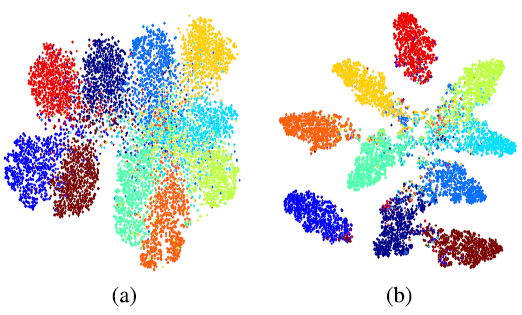
\includegraphics[scale=0.60]{images/04_1.png}
    \caption{Example of t-SNE visualization. (a) without t-SNE. (b) with t-SNE.}
    \label{fig:04_1}
\end{figure}

\FloatBarrier
    \chapter{Rotation Invariant Local Binary Convolution Neural Networks}

{\small \textbf{Authors}\\
XIN ZHANG, YUXIANG XIE, JIE CHEN, (Member, IEEE), LINGDA WU, QIXIANG YE, (Senior Member, IEEE), AND LI LIU\\ \\
IEEE Access\\VOLUME 6, 2018}

\section{Proposed Method}
 
Despite what it has been seen in the previous paper, the problem of the feature invariance is covered also here but with a very different approach. In fact, previously it has been dealt more with distances in manifolds representing classes. On the other hand, in this paper, a new architecture for CNNs is proposed, whose aim is to increase the ability of our network to handle features invariance. The problem itself is how to deal with objects that might change in position and more. It is worth pointing out that some of the advice given in this paper are in disagreement with the previous one. For example, data augmentation has been slightly criticized before, because it does not improve more than 1\% performance if we increase training samples from 1M to 14M. On the other hand, in the following work it is highly recommended. Moreover, data augmentation can be pursued through two different approaches. The first one seems to be the handcrafted design of the features we are looking for but it is such a heavy and slow process and is not that efficient. Otherwise, there is the classical approach to perform basic operations to enlarge our dataset, where we end up with a higher invariance. As this is only a precondition, let us see now what is the proposed method about. A new CNN is proposed and it is called \textit{Rotation Invariant Local Binary Convolutional Neural Network} (RI-LBCNN) that basically is a new architecture in which a module is added. This module is the \textit{Local Binary orientation Module} (LBoM). The main difference between a common CNN and a LBCNN is that the convolutional layer is replaced with something called Local Binary Convolution (LBConv) that is able to achieve the same performance of CNNs but with fewer parameters. The following module is made of three layers. The first two make up the first component, while the other layer makes up the second one. More specifically, what is done in this module is to use binary filters that we initialize through a Bernoulli distribution. At the same time, while we are performing the convolution operation, we properly rotate these filters in order to obtain other orientation channels. An illustration of the whole module architecture is shown in Figure \ref{fig:05_1}. As we can see, in the first component, there are the two mentioned layers where through activations we end up with bit maps, then we move to the second component where features maps are obtained as output.\\

\begin{figure}[h!]
    \centering
    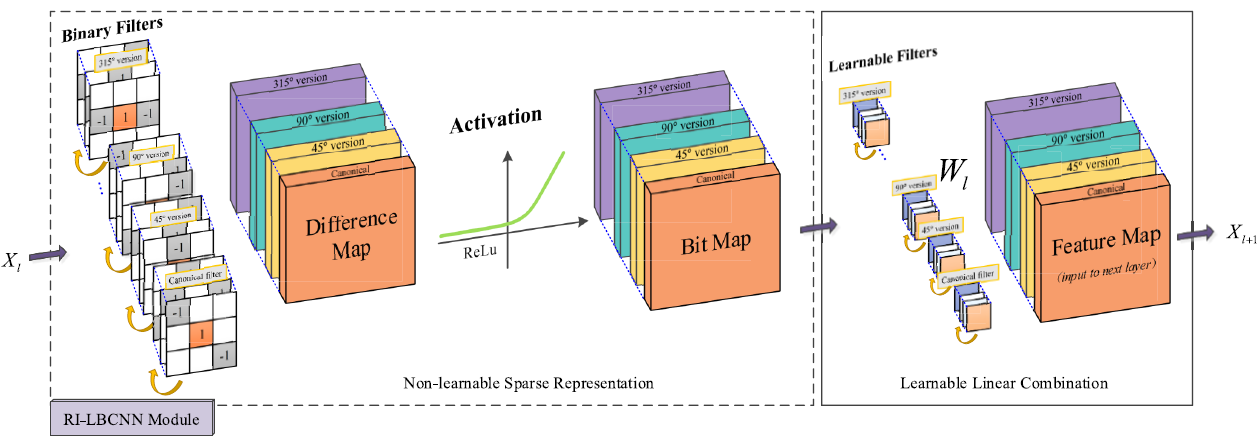
\includegraphics[scale=0.45]{images/05_1.png}
    \caption{Local Binary orientation Module (LBoM) in RI-LBCNNs.}
    \label{fig:05_1}
\end{figure}

\FloatBarrier
 
\section{Experimental Results}

Let us now move into experimental results. The datasets used here are the MNIST \citep{MNIST} and other two its variants that are MNIST-rot-12k and MNIST-rot. These two variants are still based on the original MNIST but they are built in order to better face the rotation-variant problem. After having carried out a few tests, some among the most known CNN architectures such as VGGNet, ResNet and WideResNet are used to deal with an image classification problem with other two datasets that are CIFAR10 \citep{CIFAR10and100} and CIFAR100 \citep{CIFAR10and100}. It turns out that CNNs using the proposed LBoM module outperform the aforementioned architectures that do not use it. 

    \chapter{Low-Complexity Approximate Convolutional Neural Networks}

{\small \textbf{Authors}\\
Renato J. Cintra, \textit{Senior Member, IEEE}, Stefan Duffner, Christophe Garcia, and André Leite\\ \\
IEEE TRANSACTIONS ON NEURAL NETWORKS AND LEARNING SYSTEMS\\VOL. 29, NO. 12, DECEMBER 2018}

\section{Proposed Method}

As we have already seen in most of the papers discussed, the main goal is to improve performance of our networks. In the following paper, we are going to discuss about another approach whose aim is to reduce the complexity of the CNN used. An important difference this time is that the purpose of this study is not to achieve the state-of-the-art, while it is to present an effective way to reduce a lot the number of the parameters, and by doing so, we end up with a lighter architecture that can be more easily employed by systems with limited hardware resources.\\ \\
The basic idea in the proposed method is to replace all the multiplication operations usually performed into the convolution matrices with simple additions and bit-shifting operations. In order to achieve that, we come up with an optimization problem in which we aim at obtaining an approximated matrix $\hat{\textbf{M}}$ that will be such that $\textbf{M} \approx \hat{\textbf{M}}$. Where $\textbf{M}$ is the matrix that we would obtain without any approximation in a conventional CNN. There are a few things that would be worth saying more about. For example, the Frobenius norm is used as way to express the idea of distance seen as the difference between the two matrices abovementioned. The Frobenius norm is basically the square root of the sum of all the absolute values of our matrix, squared.

\section{Experimental Results}

Experimental results have been evaluated on two different applications: face detection and digit recognition. The first one is a binary classification, where we are basically trying to understand whether or not an image has a face in some region. Results show that by applying the proposed model we end up with almost the same accuracy of a baseline model such as a face detector called CFF but with fewer parameters and with operations performed optimally. The second application, digit recognition, is evaluated through the typical dataset MNIST \citep{MNIST}. Also in this case the multiplications have been replaced by additions and bit-shifting and this is translated into an approximation even better than that seen for the binary classification.

    \chapter{Convolution in Convolution for Network in Network}

{\small \textbf{Authors}\\
Yanwei Pang, \textit{Senior Member, IEEE}, Manli Sun, Xiaoheng Jiang, and Xuelong Li, \textit{Fellow, IEEE}\\ \\
IEEE TRANSACTIONS ON NEURAL NETWORKS AND LEARNING SYSTEMS\\VOL. 29, NO. 5, MAY 2018}

\section{Proposed Method}

In the following paper we are going to talk about another type of CNN. The proposed method comes from another architecture called \textit{Network in Network} (NiN). The main difference between a NiN and a conventional CNN is that the linear filter is replaced by a \textit{multilayer perceptron} (MLP). As a MLP is a nonlinear activation function and we are replacing a filter that is linear, we can consider the MLP as a small network. Another evident difference is that by employing MLP we end up having a very dense connected structure, while previously with filters, we had a shared approach.\\ \\
The proposed method here is called \textit{Convolution in Convolution} (CiC) and is an improved version of NiN. In CiC, an unshared convolution is applied on the \textit{depth} (that is like applying a sparsification on connections), while a shared convolution is applied on the spatial domain (\textit{$width \times height$}). As it turned out from other papers, sparsifying is a good idea when we want to reduce both the overfitting and the number of the parameters as well as it has done here. As regards the difference between a NiN and the proposed CiC, we have that in a CiC, the MLPs (that are used as filters in NiNs) are divided into two categories: \textit{fully sparse MLP} and \textit{partially sparse MLP}. In order to have a more precise idea of what they are, we show their representation in Figure \ref{fig:07_1}. It turns out that the best configuration is the MLP-dense-sparse-dense because it is not possible to have sparsification in the first layer. Moreover, for the sake of the clarity, in the shown image, '0' means dense (fully-connected) and '1' means sparse.\\

\begin{figure}[h!]
    \centering
    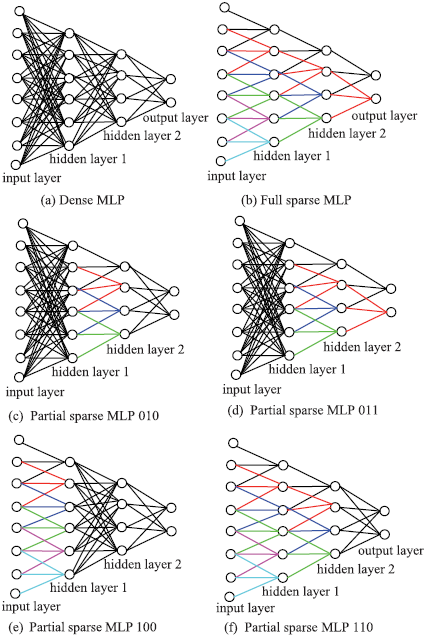
\includegraphics[scale=0.85]{images/07_1.png}
    \caption{(a) Fully connected MLP. (b) Full sparse MLP. (c)–(e) Different types of partial sparse MLPs.}
    \label{fig:07_1}
\end{figure}

\FloatBarrier

\section{Experimental Results}

Experimental results have been evaluated using two structures on different architectures and datasets. Also here data augmentation is performed and in this case we end up having different versions of the original datasets. More specifically, CIFAR10 \citep{CIFAR10and100} and CIFAR100 \citep{CIFAR10and100} become CIFAR10+, CIFAR10++ and CIFAR100+. The two abovementioned structures are respectively: CiC-1-D and CiC-3-D. The difference between them is that in the first one, the convolution (in the spatial domain) is performed with a $1 \times 1$ filter (and in one dimension as regards the depth), while in the second one we increase the size to $n \times n$ and we consider three dimensions filtering. Both structures behave well on the provided datasets, in fact they achieve very good test error rates that validate the following method. 

    \chapter{Generalizing Pooling Functions in CNNs: Mixed, Gated, and Tree}

{\small \textbf{Authors}\\
Chen-Yu Lee, Patrick Gallagher and Zhuowen Tu\\ \\
IEEE TRANSACTIONS ON PATTERN ANALYSIS AND MACHINE INTELLIGENCE\\VOL. 40, NO. 4, APRIL 2018}

\section{Proposed Method}

The pooling layer has already been presented in the overview of this report but here we will talk about it going more in depth. The pooling operation is usually employed in CNNs because downsamples the feature maps ending up with smaller resolutions, and for this reason is quite convenient to use it because we aim at gradually reducing the size of our layers while we move through them. There are a few pooling operations but in this paper we will take into account mainly two of them: the \textit{max} and the \textit{average} pooling. In the first one we take the max over 4 numbers (if we have $2 \times 2$ regions in some depth). In the second one we take the average. It should be noted that the depth dimension remains the same. More specifically, in the following paper, we will propose two approaches to generalize pooling. The first approach is split into two strategies that are respectively: \textit{mixed max-average pooling} and \textit{gated max-average pooling}. As our main goal is to obtain a good responsiveness into our pooling functions, we will decide if these two strategies are responsive or unresponsive depending on how well they are able to generalize. Mixed max-average pooling, is said to be unresponsive because it is only a standard combination of max and average pooling and it does not react to the features of the pooled region. On the other hand, in gated max-average pooling, we notice a responsiveness to changes in the pooled region. After having pointed out this main difference, let us explain how they both are implemented. As far as the mixed max-average pooling, we have a parameter called $a$ that is defined between 0 and 1 and basically is a scalar that allows us to balance the amount of max pooling and average pooling into our general equation that is:

\begin{equation}
    \label{eq:08_1}
    f_{mix}(\textbf{x}) = a_{\ell} \cdot f_{max}(\textbf{x})+(1- a_{\ell}) \cdot f_{avg}(\textbf{x})
\end{equation}\\
In gated max-average pooling instead, we are still trying to learn a proportion but this time we use a gating mask that is multiplied with the region we mean to pool and the result is used to apply a sigmoid activation function. In Figure \ref{fig:08_1} we show an illustration of both methods.\\

\begin{equation}
    \label{eq:08_2}
    f_{gate}(\textbf{x}) = \sigma(\mathbold{\omega}^T\textbf{x})f_{max}(\textbf{x})+(1-\sigma(\mathbold{\omega}^T\textbf{x}))f_{avg}(\textbf{x})
\end{equation}

\begin{figure}[h!]
    \centering
    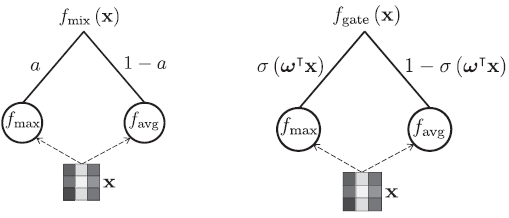
\includegraphics[scale=0.75]{images/08_1.png}
    \caption{Left: mixed max-average pooling. Right: gated max-average pooling.}
    \label{fig:08_1}
\end{figure}

\FloatBarrier

Another way to understand how to generalize pooling, is by combining its operations between them in order to learn the parameters that we need in the filters by themselves. How we can do that? We use trees. More specifically we use decision trees whose aim is to learn filters and how they can be combined. To better understand how they work we provide an illustration as shown in Figure \ref{fig:08_2}

\begin{figure}[h!]
    \centering
    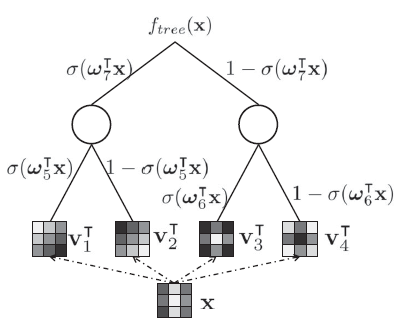
\includegraphics[scale=0.65]{images/08_2.png}
    \caption{Tree pooling operation.}
    \label{fig:08_2}
\end{figure}

\FloatBarrier

As we can see, this tree has three levels and each leaf is a filter we want to learn. If we have only one node we end up with only $\textbf{v}_m^T \textbf{x}$. Instead, if we have more nodes, we combine the result of both left and right children with the strategy presented in gated max-average pooling.

\section{Experimental Results}

Experiments have been conducted on five datasets. They are MNIST \citep{MNIST}, CIFAR10 \citep{CIFAR10and100}, CIFAR100 \citep{CIFAR10and100}, SVHN \citep{SVHN} and ImageNet \citep{ImageNet12}. It turns out that by applying the proposed methods we must sacrifice the time execution by a range of 5-15\%. But it has been proved that it is not a big issue as it is quite easy to implement and it is worth it. In order to achieve better performance, the usual data augmentation has been employed and also batch normalization as far as regularization tecniques. Final results show that the state-of-the-art is achieved on three out five abovementioned datasets. This would suggest the effectiveness of the proposed pooling operations. 



    \chapter{Low Complexity Multiply Accumulate Unit for Weight-Sharing Convolutional Neural Networks}

{\small \textbf{Authors}\\
James Garland and David Gregg\\ \\
IEEE COMPUTER ARCHITECTURE LETTERS\\VOL. 16, NO. 2, JULY-DECEMBER 2017}

\section{Proposed Method}

This is the first paper in which we are going to discuss about something that deals with both hardware and the pure model. Until now, we have been discussing only about technical improvements related to CNNs from a modeling perspective. For instance, we have talked a lot about number of layers, size of filters, pooling operations, how to better convolve etc. On the other hand here, we will debate on advantages of adopting a different tecnique to store weights, that is closer to the hardware. The idea is to propose a different way to perform the accumulation of the weights in the \textit{Multiply Accumulate Unit} (MAC). Recall that the multiply accumulate operation is the product between two numbers where the result is added to an accumulator, which is also known as Sum of Products (SOP). So instead of doing that, a different approach is proposed. Basically, for each weight that we have, we put its image (that is different from its original value) into a bucket with a fixed index. Until weights show up, we add their images to the right buckets. What we are doing is performing an accumulation. The next step now is to perform the multiplication between the image values stored into our buckets and the value of the weight of that bucket. By doing so we reduce a lot the number of operations that we should have done because we move from a multiplication accumulation problem to an addition based on array indexes. As this might be a little difficult to imagine, we provide an illustration of these accumulators in Figures \ref{fig:09_2} and \ref{fig:09_3}.\\

\begin{figure}[h!]
    \centering
    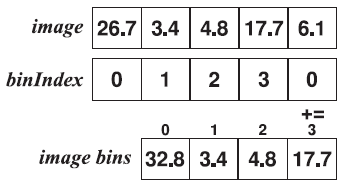
\includegraphics[scale=0.70]{images/09_2.png}
    \caption{Step 1: Accumulation of images.}
    \label{fig:09_2}
\end{figure}

\FloatBarrier

\begin{figure}[h!]
    \centering
    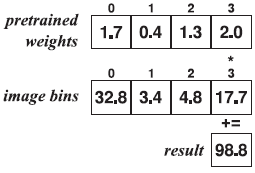
\includegraphics[scale=0.70]{images/09_3.png}
    \caption{Step 2: Multiplication between the values of the weights and the corresponding accumulated value.}
    \label{fig:09_3}
\end{figure}

\FloatBarrier

\section{Experimental Results}

As far as experimental results it is necessary to point some things out. First of all no dataset has been mentioned in the paper. Moreover, we are going to spend a few words on what turned out by doing a couple of tests. Some parameters have been compared, such as how big was the impact of the proposed architecture on not so powerful devices and also how many gates have been used to perform the desired logic on the MAC. As we do not mean to draw conclusions on things not directly related to our sphere of competence we will not compare these parameters. On the other side, it has been shown that we have to pick very carefully the number of the buckets because above a certain value, performance gets worse. All in all, if we choose with care the number of buckets that in the paper are called bins, we achieve better results than the classic MAC unit.
    \chapter{StochasticNet: Forming Deep Neural Networks via Stochastic Connectivity}

{\small \textbf{Authors}\\
MOHAMMAD JAVAD SHAFIEE, (Student Member, IEEE), PARTHIPAN SIV, AND ALEXANDER WONG, (Senior Member, IEEE)\\ \\
IEEE ACCESS\\VOLUME 4, 2016}

\section{Proposed Method}

This is going to be the last paper we will be discussing in this report and what we want to do is to make a comparison between the following proposed method and some regularization tecniques. So far we have mentioned many times Dropout and Batch Normalization as well as DisturbLabel and most likely something else. The important thing to point out is that with StochasticNet (which is the name of the proposed network) we are not talking about a specific regularization tecnique but as there are a few things in common it is actually possible to make a comparison. Before of going any further it would make sense to introduce the topic from which the StochasticNet comes from and it is the theory by which a neural network can be represented as a random graph. Obviously in this graph there are many constraints as it is not possible to have that neurons in a layer are connected with neurons of non-adjacent layers, and moreover, as we are presenting a stochastic network, it must be clear that when we create a connection between two nodes (or neurons) there is a constraint that shall be such that the weight is between 0 and 1. So we look at weights as if they were probabilities. What we can do in StochasticNets is to set a value that represents the sparsity (the probability by which is possible to create a connection) we are looking for and then we can understand how different performance is when testing the network on some datasets. But we will compare these things in the following section. The important thing is to understand that while with a regularization tecnique such as Dropout we temporarily ``freeze'' the values of the weights (by setting them to zero) during the training step, here with StochasticNet we start with a sparse network and finish with a sparse network. In fact, after a regularization tecnique is employed, it is applied only in the training step. When the training is done, we resume the frozen weights and use the full network with the test set. That does not happen with StochasticNet. In order to get a better idea, we show in Figure \ref{fig:10_2} the several phases of a model through different regularization tecniques and of course StochasticNet.\\

\begin{figure}[h!]
    \centering
    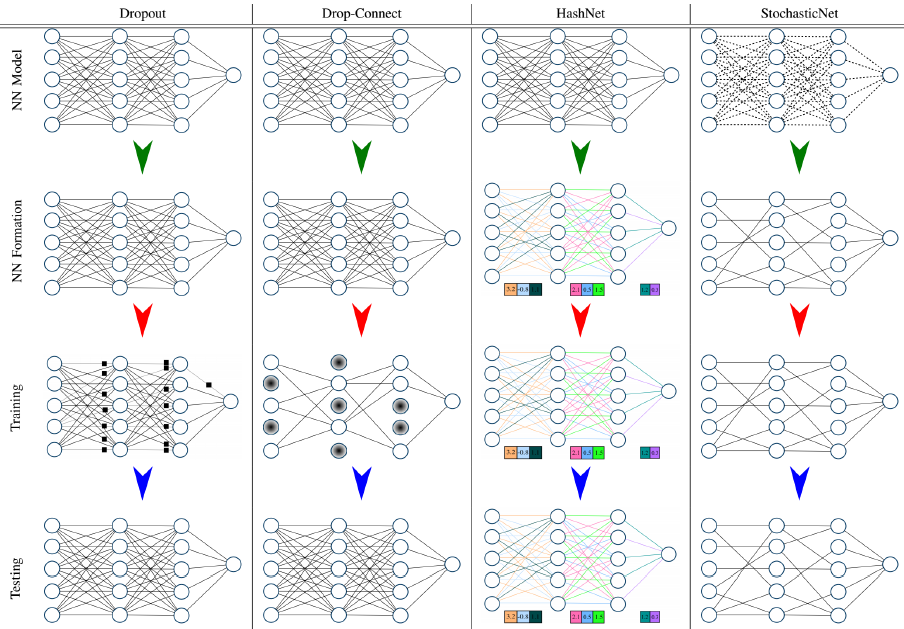
\includegraphics[scale=0.60]{images/10_2.png}
    \caption{Comparison among several stochastic regularization methods and StochasticNet.}
    \label{fig:10_2}
\end{figure}

\FloatBarrier

\section{Experimental Results}

Experimental results have been evaluated on the following datasets: CIFAR-10 \citep{CIFAR10and100}, MNIST \citep{MNIST}, SVHN \citep{SVHN} and STL-10 \citep{STL10}. After having performed a few tests it turns out that StochasticNet achieves the same test error of a conventional CNN but with far fewer connections. In fact, it is estimated that we have around half of the connections. Moreover, we can justify the following results as in the convolution, we perform the dot product between the filter and the matrix with a sparsified matrix. On the other hand in an ordinary CNN we have a non-sparse matrix. That is why it can be translated into a very good improvement, even though a degradation of our performance is obtained once we go below the 39\% of connectivity. But it seems to be quite reasonable and it still confirms the effectiveness of this network.
    
    % Conclusion
    \chapter{Conclusion}

Let us briefly recap what has been shown during this report. The main focus has been on \textit{Convolutional Neural Networks}. Several tecniques and different approaches have been proposed to improve performance of CNNs. We have firstly talked about what CNNs are and what their building blocks are. Then, we introduced some methods whose aim was to improve their accuracy on test sets. We used a few datasets such as MNIST \citep{MNIST}, CIFAR10 \citep{CIFAR10and100}, CIFAR100 \citep{CIFAR10and100}, STL10 \citep{STL10}, ImageNet \citep{ImageNet12}, LFW \citep{LFW}, Outex \citep{Outex} and SVHN \citep{SVHN}. They all were really important to compare different results achieved using different network architectures. Let us now dive into what we have seen while discussing about these papers.\\ \\
It seems to be clear that a CNN can be created by choosing a bunch of different parameters. That is why many researchers came up with several different architectures. Some of them have been more concentrated on how deep the neural network was supposed to be, going from a few layers to thousands of them. On the other hand, others have been more focused on how to ease the convolution operation. Also several activation functions were proposed. It is worth to mention the classic sigmoid which is almost every time replaced by the ReLU today (or also its slight variant Leaky ReLU). Some of the studies covered, showed that in order to extract more complex features, a few tricks can be used. We mention the data augmentation that basically allows the model to better abstract extracted features. For instance, some basic operation such as cropping, flipping etc. have been performed on almost all the datasets mentioned before. This allows the model to capture also different angles and lighting conditions of the image provided as input to the classificator which increases a lot the final accuracy. Moreover, some comments have been made on the output layer of a CNN and how to increase nonlinearity in order to better discriminate final classes. We have seen that, despite in CNNs we do not have all neurons connected with their former layer, in the last layer we need to have this configuration. Some other approaches proposed to have sparser networks by performing some regularization operations such as dropout or batch normalization. We also saw different pooling functions, in order to better downsample the input image while going deeper in the network. Finally, we discussed about a hardware accelerator that could help to obtain faster CNNs in order to deploy them also on mobile systems which can not substain the computational power usually required to run these models.\\ \\
We can conclude by saying that several were the proposed methods for CNNs, but in the end, when dealing with a problem (in this case it is image classification/object detection) we need to reach a compromise. Some of these papers have pointed out that it does not make totally sense to go deeper with more layers if this means that we are complicating the structure of the network. Because it would only be a race where the most powerful hardware achieves better results. Instead, it would make more sense to improve the local block of the whole architecture, as we have seen by comparing some of the previous papers.
    
    % References
    \renewcommand{\bibname}{References}

\bibliographystyle{plain}
\bibliography{references}

\end{document}
